%\documentclass[icelandic]{beamer}

\documentclass[icelandic,a4paper,12pt]{article}
\usepackage{beamerarticle}

\mode<presentation>
{
  \usetheme{boxes}
  % með efnisyfirliti: Szeged, Frankfurt 
  % án efnisyfirlits: Pittsburgh
  % áhugavert: CambridgeUS, Boadilla
  %\setbeamercovered{transparent} %gegnsætt
  \setbeamercovered{invisible}
  }

\usepackage[english,icelandic]{babel}
\usepackage[utf8]{inputenc}
\usepackage{t1enc}
\selectlanguage{icelandic}
\usepackage{graphicx}
\usepackage{amsmath}
\usepackage{amssymb}
\usepackage{mathrsfs}
% \newcommand{\C}{{\mathbb  C}}
% \newcommand{\Z}{{\mathbb Z}}
% \newcommand{\R}{{\mathbb  R}}
% \newcommand{\N}{{\mathbb  N}}
% \newcommand{\Q}{{\mathbb Q}}
\renewcommand{\phi}{\varphi}
\renewcommand{\epsilon}{\varepsilon}

%\usepackage{pgfpages}
% \pgfpagesuselayout{2 on 1}[a4paper,border shrink=5mm]

\def\lecturename{Stærðfræðigreining IB}
\title{\insertlecture}
\author{Benedikt Steinar Magnússon, \href{mailto:bsm@hi.is}{bsm@hi.is}}
\institute
{
  Verkfræði- og náttúruvísindasvið\\
  Háskóli Íslands
}
\subtitle{Stærðfræðigreining IB}
%\subject{\lecturename}

\mode<article>
{
	\usepackage[colorlinks=false,
	pdfauthor={Benedikt Steinar Magnusson},
	pdftitle={IB: Namsefni
	}]{hyperref}
  %\usepackage{times}
  %\usepackage{mathptmx}
  \usepackage[left=1.5cm,right=4cm,top=1.5cm,bottom=3cm]{geometry}
}

% Beamer version theme settings

%\useoutertheme[height=0pt,width=2cm,right]{sidebar}
%\usecolortheme{rose,sidebartab}
%\useinnertheme{circles}
%\usefonttheme[only large]{structurebold}

\setbeamercolor{sidebar right}{bg=black!15}
\setbeamercolor{structure}{fg=blue}
\setbeamercolor{author}{parent=structure}

\setbeamerfont{title}{series=\normalfont,size=\LARGE}
\setbeamerfont{title in sidebar}{series=\bfseries}
\setbeamerfont{author in sidebar}{series=\bfseries}
\setbeamerfont*{item}{series=}
\setbeamerfont{frametitle}{size=}
\setbeamerfont{block title}{size=\small}
\setbeamerfont{subtitle}{size=\normalsize,series=\normalfont}

\defbeamertemplate*{footline}{infolines theme}
 {
   \leavevmode%
   \hbox{%
   \begin{beamercolorbox}[wd=.333333\paperwidth,ht=2.25ex,dp=1ex,center]{author in head/foot}%
   %  \usebeamerfont{author in head/foot}\insertshortauthor~~\beamer@ifempty{\insertshortinstitute}{}{(\insertshortinstitute)}
   \end{beamercolorbox}%
   \begin{beamercolorbox}[wd=.333333\paperwidth,ht=2.25ex,dp=1ex,center]{title in head/foot}%
    % \usebeamerfont{title in head/foot}\insertshorttitle
   \end{beamercolorbox}%
   \begin{beamercolorbox}[wd=.333333\paperwidth,ht=2.25ex,dp=1ex,right]{date in head/foot}%
     %\usebeamerfont{date in head/foot}\insertshortdate{}\hspace*{2em}
     \insertshortlecture.\insertframenumber{} / \insertshortlecture.\inserttotalframenumber\hspace*{2ex} 
   \end{beamercolorbox}}%
   \vskip0pt%
 }
  


\setbeamertemplate{sidebar right}
{
  {\usebeamerfont{title in sidebar}%
    \vskip1.5em%
    \hskip3pt%
    \usebeamercolor[fg]{title in sidebar}%
    \insertshorttitle[width=2cm-6pt,center,respectlinebreaks]\par%
    \vskip1.25em%
  }%
  {%
    \hskip3pt%
    \usebeamercolor[fg]{author in sidebar}%
    \usebeamerfont{author in sidebar}%
    \insertshortauthor[width=2cm-2pt,center,respectlinebreaks]\par%
    \vskip1.25em%
  }%
  \hbox to2cm{\hss\insertlogo\hss}
  \vskip1.25em%
  \insertverticalnavigation{2cm}%
  \vfill
  \hbox to 2cm{\hfill\usebeamerfont{subsection in
      sidebar}\strut\usebeamercolor[fg]{subsection in
      sidebar}\insertshortlecture.\insertframenumber\hskip5pt}%
  \vskip3pt%
}%

\setbeamertemplate{title page}
{
  \vbox{}
  \vskip1em
  %{\huge Kapitel \insertshortlecture\par}
  {\usebeamercolor[fg]{title}\usebeamerfont{title}\inserttitle\par}%
  \ifx\insertsubtitle\@empty%
  \else%
    \vskip0.25em%
    {\usebeamerfont{subtitle}\usebeamercolor[fg]{subtitle}\insertsubtitle\par}%
  \fi%     
  \vskip1em\par
  %Vorlesung \emph{\lecturename}\ vom 
  \insertdate\par
  \vskip0pt plus1filll
  \leftskip=0pt plus1fill\insertauthor\par
  \insertinstitute\vskip1em
}

%\logo{\includegraphics[width=2cm]{beamerexample-lecture-logo.pdf}}



% Article version layout settings

\mode<article>

\makeatletter
\def\@listI{\leftmargin\leftmargini
  \parsep 0pt
  \topsep 5\p@   \@plus3\p@ \@minus5\p@
  \itemsep0pt}
\let\@listi=\@listI


\setbeamertemplate{frametitle}{\paragraph*{\insertframetitle\
    \ \small\insertframesubtitle}\ \par
}
\setbeamertemplate{frame end}{%
  \marginpar{\scriptsize\hbox to 1cm{\sffamily%
      \hfill\strut\insertshortlecture.\insertframenumber}\hrule height .2pt}}
\setlength{\marginparwidth}{1cm}
\setlength{\marginparsep}{1.5cm}

\def\@maketitle{\makechapter}

\def\makechapter{
  \newpage
  \null
  \vskip 2em%
  {%
    \parindent=0pt
    \raggedright
    \sffamily
    \vskip8pt
    %{\fontsize{36pt}{36pt}\selectfont Kapitel \insertshortlecture \par\vskip2pt}
    {\fontsize{24pt}{28pt}\selectfont \color{blue!50!black} \insertlecture\par\vskip4pt}
    {\Large\selectfont \color{blue!50!black} \insertsubtitle, \@date\par}
    \vskip10pt

    \normalsize\selectfont \@author\par\vskip1.5em
    %\hfill BLABLA
  }
  \par
  \vskip 1.5em%
}

\let\origstartsection=\@startsection
\def\@startsection#1#2#3#4#5#6{%
  \origstartsection{#1}{#2}{#3}{#4}{#5}{#6\normalfont\sffamily\color{blue!50!black}\selectfont}}

\makeatother

\mode
<all>




% Typesetting Listings

\usepackage{listings}
\lstset{language=Java}

\alt<presentation>
{\lstset{%
  basicstyle=\footnotesize\ttfamily,
  commentstyle=\slshape\color{green!50!black},
  keywordstyle=\bfseries\color{blue!50!black},
  identifierstyle=\color{blue},
  stringstyle=\color{orange},
  escapechar=\#,
  emphstyle=\color{red}}
}
{
  \lstset{%
    basicstyle=\ttfamily,
    keywordstyle=\bfseries,
    commentstyle=\itshape,
    escapechar=\#,
    emphstyle=\bfseries\color{red}
  }
}



% Common theorem-like environments

\theoremstyle{definition}
\newtheorem{exercise}[theorem]{\translate{Exercise}}




% New useful definitions:

\newbox\mytempbox
\newdimen\mytempdimen

\newcommand\includegraphicscopyright[3][]{%
  \leavevmode\vbox{\vskip3pt\raggedright\setbox\mytempbox=\hbox{\includegraphics[#1]{#2}}%
    \mytempdimen=\wd\mytempbox\box\mytempbox\par\vskip1pt%
    \fontsize{3}{3.5}\selectfont{\color{black!25}{\vbox{\hsize=\mytempdimen#3}}}\vskip3pt%
}}

\newenvironment{colortabular}[1]{\medskip\rowcolors[]{1}{blue!20}{blue!10}\tabular{#1}\rowcolor{blue!40}}{\endtabular\medskip}

\def\equad{\leavevmode\hbox{}\quad}

\newenvironment{greencolortabular}[1]
{\medskip\rowcolors[]{1}{green!50!black!20}{green!50!black!10}%
  \tabular{#1}\rowcolor{green!50!black!40}}%
{\endtabular\medskip}



\lecture[1]{2. Markgildi og samfelldni}{lecture-text}
\date{29. ágúst 2015}

\newcommand{\C}{{\mathbb  C}}
\newcommand{\Z}{{\mathbb Z}}
\newcommand{\R}{{\mathbb  R}}
\newcommand{\N}{{\mathbb  N}}
\newcommand{\Q}{{\mathbb Q}}
\newcommand{\Sin}{{\text{Sin}}}
\newcommand{\Tan}{{\text{Tan}}}
\newcommand{\Cos}{{\text{Cos}}}
\newcommand{\Cosh}{{\text{Cosh}}}
\newcommand{\arsinh}{{\text{arsinh}}}
\newcommand{\arcosh}{{\text{arcosh}}}
\newcommand{\artanh}{{\text{artanh}}}


\begin{document}
\setcounter{tocdepth}{2}
\tableofcontents


\section{Könnun falla}

\subsection{Inngangur}
\subsubsection{Frávik frá bókinni}
Það sem á eftir kemur er eitt af fáum atriðum þar sem
mín nálgun og skilgreiningar eru frábrugðnar þeim í 
bókinni.

\subsubsection{Hver er munurinn?}
\begin{center}
\begin{columns}[c] % contents are top vertically aligned 
\begin{column}{.5\textwidth}
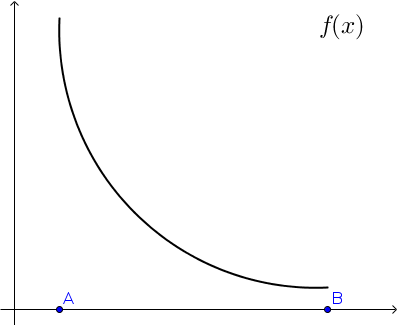
\includegraphics[width=6cm,keepaspectratio=true]{./myndir/kafli05/01_f1.png}
\end{column}
\begin{column}{.5\textwidth}
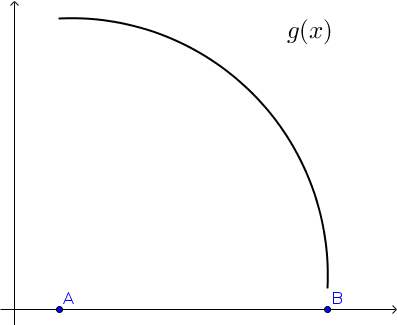
\includegraphics[width=6cm,keepaspectratio=true]{./myndir/kafli05/01_g1.png}
\end{column}
\end{columns}
\end{center}
\subsubsection{}
Skoðum föllin tvö að ofan,
þau eru augljóslega ekki eins, þannig að spurningin er hvernig getum
við lýst því muninum á þeim?

Þau hugtök sem við höfum skoðað hingað til geta ekki greint á milli
þessara falla:
\begin{enumerate}[(i)]
\item Þau hafa sama skilgreiningarmengið $[A,B]$\pause
\item Þau taka sömu gildin í endapunktunum\pause
\item Þau hafa bæði hágildi í $A$ og lággildi í $B$\pause
\item Þau eru bæði minnkandi \pause (neikvæð afleiða)
\end{enumerate}

 


\subsubsection{Drögum sniðil}
\begin{columns}[c] % contents are top vertically aligned 
\begin{column}{.5\textwidth}
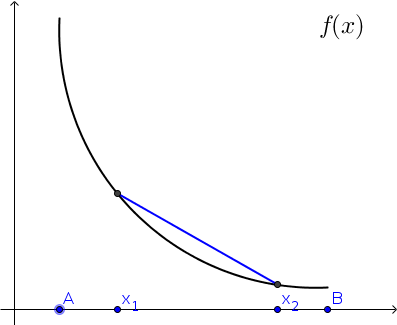
\includegraphics[width=6cm,keepaspectratio=true]{./myndir/kafli05/01_f2.png}
\end{column}
\begin{column}{.5\textwidth}
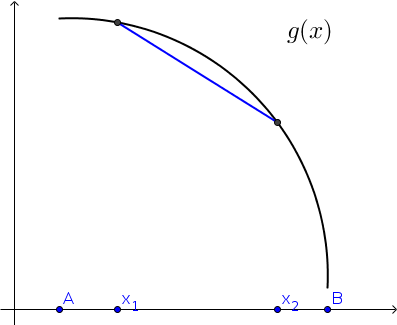
\includegraphics[width=6cm,keepaspectratio=true]{./myndir/kafli05/01_g2.png}
\end{column}
\end{columns}
Ef við veljum nú tvo punkta á $[A,B]$ af handahófi, köllum þá $x_1$ og $x_2$, og drögum línu (sniðil)
í gegnum punktana á grafum $f$ og $g$ þá sjáum við 
að sniðillinn lendir fyrir neðan $g$ en ofan $f$.
 
Sérhvern punkt á milli $x_1$ og $x_2$, getum við skrifað $\alpha x_1 + (1-\alpha)x_2$, $\alpha \in [0,1]$. Þá er $y$-hnit punktsins á sniðlinum með þetta $x$-hnit gefið með 
$$
	\alpha f(x_1) + (1-\alpha) f(x_2), \qquad \alpha \in [0,1],
$$
á fyrri myndinni og 
$$
	\alpha g(x_1) + (1-\alpha) g(x_2), \qquad \alpha \in [0,1],
$$
á myndinni fyrir $g$


Ef $f$ liggur fyrir neðan sniðilinn þá þýðir það að fallgildi $f$ í punktunum 
$\alpha x_1 + (1-\alpha)x_2$ liggur fyrir neðan punktinum á sniðlinum, það er
$$f(\alpha x_1+(1-\alpha)x_2)\leq \alpha f(x_1)+(1-\alpha)f(x_2).$$
Eins, ef $g$ liggur fyrir ofan sniðilinn þá gildir að
$$g(\alpha x_1+(1-\alpha)x_2)\geq \alpha g(x_1)+(1-\alpha)g(x_2).$$


\begin{columns}[c] % contents are top vertically aligned 
\begin{column}{.5\textwidth}
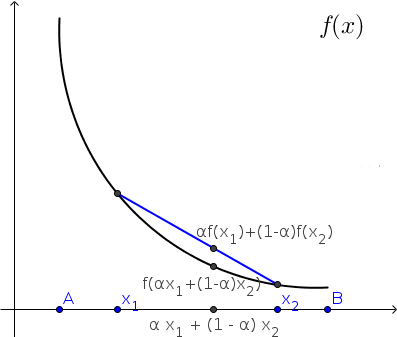
\includegraphics[width=6cm,keepaspectratio=true]{./myndir/kafli05/01_f3.png}
\end{column}
\begin{column}{.5\textwidth}
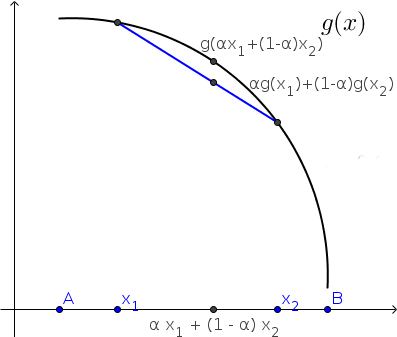
\includegraphics[width=6cm,keepaspectratio=true]{./myndir/kafli05/01_g3.png}
\end{column}
\end{columns}

\subsection{Kúpni}
\subsubsection{Skilgreining}
Látum $f:[a, b]\rightarrow \R$ vera fall.
\begin{enumerate}[(i)]\pause
\item[(i)] Segjum að fallið $f$ sé {\em kúpt} (e. convex, concave up)
ef um alla punkta $x_1, x_2\in [a, b]$ og sérhverja tölu $0\leq
\alpha\leq 1$ gildir að 
$$
	f(\alpha x_1+(1-\alpha)x_2)\leq \alpha f(x_1)+(1-\alpha)f(x_2).
$$
\pause
\item[(ii)] Segjum að fallið $f$ sé {\em hvelft} (e. concave, concave down)
ef um alla punkta $x_1, x_2\in [a, b]$ og sérhverja tölu $0\leq
\alpha\leq 1$ gildir að 
$$
	f(\alpha x_1+(1-\alpha)x_2)\geq \alpha f(x_1)+(1-\alpha)f(x_2).
$$
\end{enumerate}
 
\subsubsection{Athugasemd}
Hér fáum við hugtak sem getur útskýrt muninn á myndunum í byrjun kaflans, $f$ er kúpt og $g$ er hvelft.

\subsection{Afleiðan skoðuð nánar}
\begin{columns}[c] % contents are top vertically aligned 
\begin{column}{.5\textwidth}
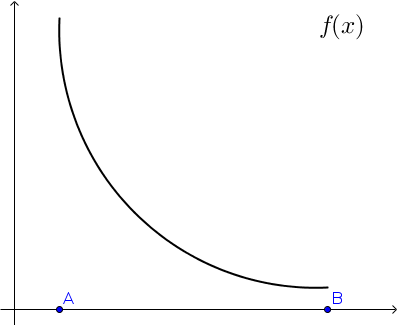
\includegraphics[width=6cm,keepaspectratio=true]{./myndir/kafli05/01_f1.png}
\end{column}
\begin{column}{.5\textwidth}
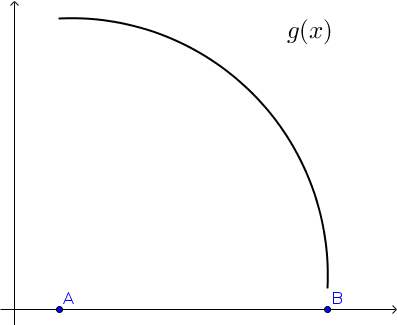
\includegraphics[width=6cm,keepaspectratio=true]{./myndir/kafli05/01_g1.png}
\end{column}
\end{columns}
\subsubsection{Athugasemd} 
Ef við skoðum afleiður fallanna $f$ og $g$ betur þá sjáum við að:
\pause
\begin{enumerate}[(i)]
\item Afleiða $f$ er mjög neikvæð nálægt $A$ og nálgast svo 0 í $B$, það er afleiðan er vaxandi.
\item Afleiða $g$ er u.þ.b.~0 í $A$ og minnkar svo þegar við nálgumst $B$, það er afleiðan er minnkandi.
\end{enumerate}
\pause
Með öðrum orðum
\pause
\begin{equation*}
	(f')' = f'' \geq 0 \qquad  \pause \text{og} \qquad
	(g')' = g'' \leq 0.
\end{equation*}

\subsection{Auðkenning á kúpni með afleiðum}
\subsubsection{Setning}
Fyrir tvídiffranlegt fall $f$ þá er eftirfarandi jafngilt
\pause
\begin{enumerate}[(i)]
\item $f$ er kúpt\pause
\item $f'$ er vaxandi\pause
\item $f'' \geq 0$
\end{enumerate}

\subsubsection{Setning}
Fyrir tvídiffranlegt fall $g$ þá er eftirfarandi jafngilt
\pause
\begin{enumerate}[(i)]
\item $g$ er hvelft\pause
\item $g'$ er minnkandi\pause
\item $g'' \leq 0$
\end{enumerate}

\subsubsection{Athugasemd}
Hvort fall er kúpt eða hvelft er {\bf algjörlega óháð} því 
hvort það er vaxandi eða minnkandi. Til dæmis er $f(x) = x^2$ kúpt en það 
er vaxandi þegar $x>0$ og minnkandi þegar $x<0$.

\subsubsection{Athugasemd}
Fall þarf eru ekki alltaf annað hvort kúpt eða hvelft alls staðar. Alveg eins og 
það eru til föll sem eru sums staðar vaxandi og sums staðar minnkandi, þá eru mörg föll
sums staðar kúpt og sums staðar hveld, til dæmis hornaföllin.

\subsection{Beygjuskilapunktar}
\subsubsection{Skilgreining}  
Punktur $(x_0, f(x_0))$ er sagður vera {\em beygjuskilapunktur}
(e.~inflection point) grafsins $y=f(x)$ ef \pause
\begin{enumerate}[(i)]
\item[(i)] grafið hefur snertilínu í $x_0$, og \pause
\item[(ii)] grafið er kúpt öðru megin við $x_0$ og hvelft hinum megin
  við $x_0$.
\end{enumerate}

\pause


\subsubsection{Setning}
Ef fallið $f$ er tvídiffranlegt þá er punkturinn $x_0$ 
beygjuskilapunktur fallsins $f$ ef og aðeins ef \pause
$f''(x_0) =0$ og $f''$ skiptir um formerki í $x_0$.
 
\begin{center}
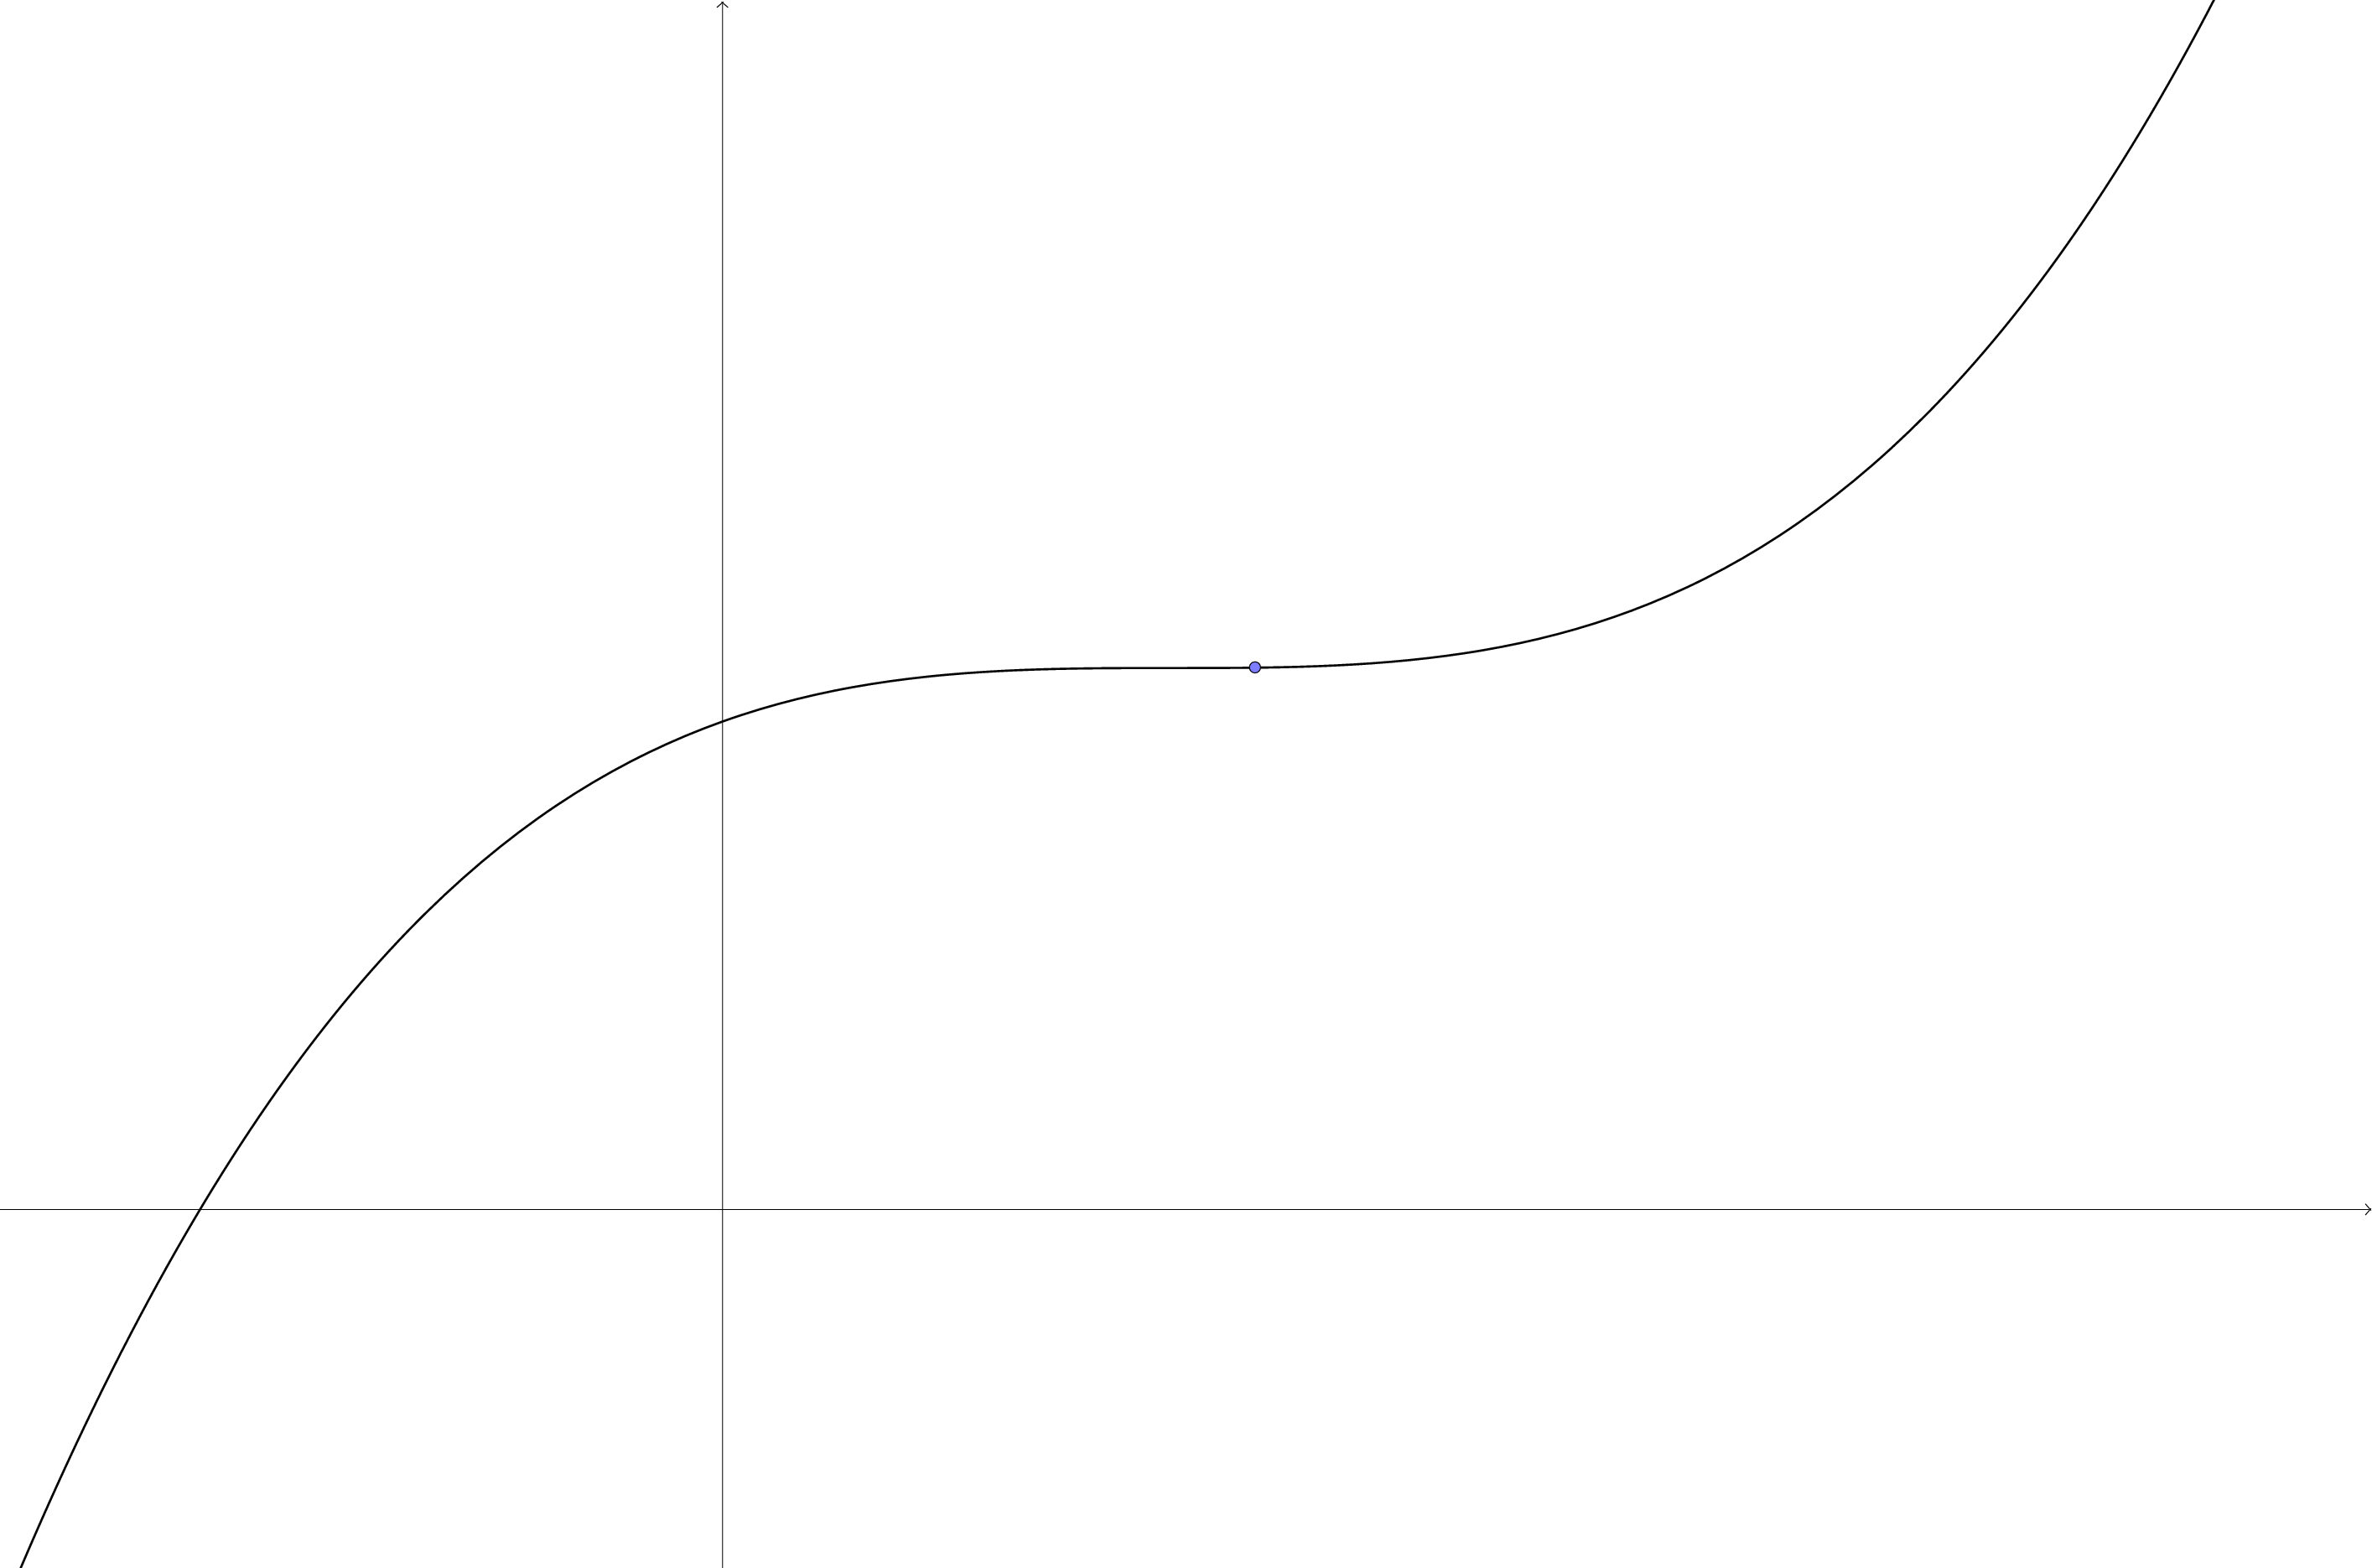
\includegraphics[width=6cm,keepaspectratio=true]{./myndir/kafli05/05_beygjuskilapunktur.png}
\end{center}


%%%%%%%%%%%%%%%%%%%%%%%%%%%%%%%%%%%%%%%%%%%%%%%%%%%%

\subsection{Útgildi}


\subsubsection{Hvar á að leita útgilda}
Sjá 
.. todo:: kafla 3
fyrir skilgreinginu á útgildi.
Punktar sem koma til greina fyrir staðbundin útgildi falls
$f$ eru\pause
\begin{enumerate}[(i)]
\item punktar $x_0$ þar sem $f'(x_0)=0$,\pause
\item punktar $x_0$ þar sem $f'(x_0)$ er ekki skilgreint,\pause
\item þeir endapunktar skilgreiningarmengisins þar sem fallið er skilgreint.
\end{enumerate}

\subsubsection{Hágildi/lágildi út frá formerki afleiðu}
Látum $x_0$ vera innri punkt á skilgreiningarsvæði $f$.  Gerum ráð
fyrir að $f$ sé diffranlegt í öllum punktum í einhverju bili utan um
$x_0$ og að $f'(x_0)=0$.
\begin{enumerate}[(i)]
\item Ef formerki $f'$ breytist úr plús í mínus í $x_0$
(farið frá vinstri til hægri eftir rauntalnaásnum) þá er
staðbundið hágildi í $x_0$.\pause
\item Ef formerki $f'$ breytist úr mínus í plús í $x_0$
þá er staðbundið lággildi í $x_0$.\pause
\item Ef formerki $f'$ breytist ekki í $x_0$ þá er hvorki 
há- né lággildi í $x_0$.   
\end{enumerate}

\subsubsection{Útgildi og önnur afleiðan}
\begin{enumerate}[(i)]
 \item Ef $f'(x_0)=0$ og $f''(x_0)<0$ þá er $x_0$ staðbundið hágildi.\pause
 \item Ef $f'(x_0)=0$ og $f''(x_0)>0$ þá er $x_0$ staðbundið lággildi.
\end{enumerate}\pause

\subsubsection{Aðvörun}
Athugið að ef $f''(x_0)=0$ þá getur $x_0$ verið hvort sem er 
staðbundið hágildi, staðbundið lággildi eða beygjuskilapunktur. 

\subsection{Aðfellur}
\subsubsection{Skilgreining: Lóðrétt aðfella}
Fallið $f$ hefur \emph{lóðrétta aðfellu} í punktinum $a$ ef 
$\lim_{x\to a^-} f(x) = \pm \infty$ og/eða
$\lim_{x\to a^+} f(x) = \pm \infty$.

Aðfellan er þá línan $x=a$.

\subsubsection{Skilgreining: Lárétt aðfella}
Fallið $f$ hefur \emph{lárétta aðfellu} ef
$\lim_{x\to \infty} f(x) = L$ og/eða
$\lim_{x\to -\infty} f(x) = L$.

Aðfellan er þá línan $y=L$.

\subsubsection{Skáfella}
Fallið $f$ hefur \emph{skáfellu} ef til eru $a$ og $b$ þannig að
$\lim_{x\to \infty} f(x) -ax-b = 0$ og/eða
$\lim_{x\to -\infty} f(x) -ax-b= 0$.

Skáfellan er þá línan $y=ax+b$.

.. todo:: myndir

\subsection{Að teikna graf falls}

.. todo:: þýða og staðfæra

 \begin{center}
 \includegraphics[width=7cm]{./myndir/kafli05/08_checklist.png}
 \end{center}
 

\subsection{Útgildisverkefni}
\subsubsection{Markmiðið}
Þessi verkefni sem við skoðum snúast um það að finna
fall fyrir stærð sem við höfum áhuga á 
(verð, rúmmál, lengd,...) og hámarka/lágmarka hana.
 
 \pause
 
Til þess að þetta sé mögulegt má fallið bara
vera háð einni breytu og það þarf helst að vera
diffranlegt.
 
 \pause
 
Þá getum við fundið útgildi með þeim aðferðum sem
við erum búin að koma okkur upp.

\subsubsection{Að leysa útgildisvandamál}
Sjá einnig bls.~259 (238 í 6.~útgáfu) í kennslubók.
\begin{enumerate}[(i)]
\item Lesið vandamálið vandlega og áttið ykkur á því
hvert það er og hvað á að finna.\pause
\item Teiknið mynd ef mögulegt er, \pause 
hún gefur oft upplýsingar um skorður sem hjálpa
okkur við að útbúa fallið.\pause
\item Skilgreinið aukabreytur.\pause
\item Skilgreinið fallið, sem fall af einni eða fleiri breytum.\pause
\item Finnið skorður (jöfnur) sem hægt er að stinga inn í fallið \pause
\item Skrifið fallið sem fall af einni breytu.\pause
\item Finnið útgildi \pause
\item Dragið ályktanir af niðurstöðunni, \pause
og athugið hvort hún sé raunhæf miðað við verkefnið (rúmmál á ekki að vera 
neikvætt og þess háttar).
\end{enumerate}
 

\subsubsection{Dæmi: Gosdós}
Hvert er hagkvæmasta formið á sívalningslaga gosdós?
\pause
\begin{center}
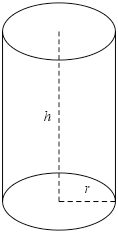
\includegraphics[width=3cm]{./myndir/kafli05/09_cylinder.png}
\end{center}

\subsubsection{Dæmi: Kassi}
Hver er stærsti (mesta rúmmálið) loklausi kassinn  sem hægt er
búa til úr örk sem er $12 \times 12$? 
\begin{center}
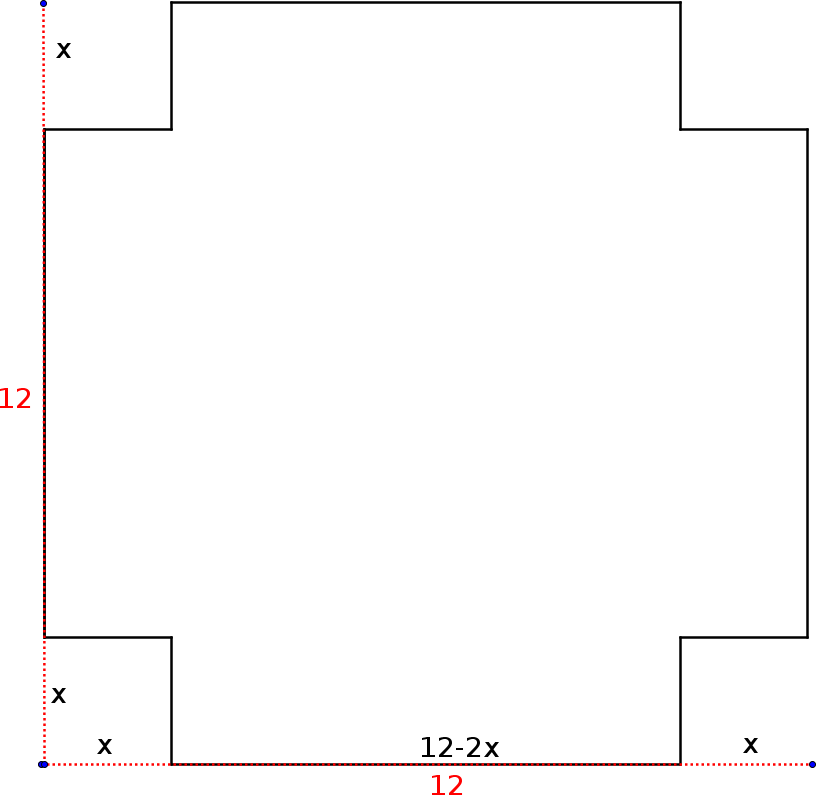
\includegraphics[width=8cm]{./myndir/kafli05/09_kassi.png}
\end{center}

\end{document}
